\documentclass{beamer}
\usetheme{Dresden}
\usepackage[utf8]{inputenc}

\title{Abschlusspräsentation}
\author{Team Ilias}
\date{\today}

\begin{document}
	\maketitle
	\frame{\tableofcontents[]}

	\section{Teamaufteilung}
	\begin{frame}
		\frametitle{Aufteilung des Teams}
		\begin{tabular}{|c|c|}\hline
			Teammitglied & Aufgabe \\\hline
			Josephine Rehak & Chefprogrammiererin\\\hline
			Richard Mörbitz & Assistent\\\hline
			Max Friedrich & Administrator\\\hline
			Peter Merseburger & Testverantwortlicher\\\hline
			Julius Felchow & Sekretär\\\hline
		\end{tabular}
	\end{frame} 
 
	\section{Aufgabe}
		\begin{frame}
			\frametitle{Einführung zur Thematik}
  			Ilias ist eine E-Learning Plattform in der E-					Klausuren erstellt werden können. Ein Fragenpool 				kann erstellt und die Fragen in der Klausur 					genutzt werden.\\
  			\pause
    		Die Reviewmöglichkeit für diese Fragen war unsere 				Aufgabe.
		\end{frame}
		\begin{frame}
			\frametitle{Aufgabenstellung}
			
		\end{frame}

		\begin{frame}
			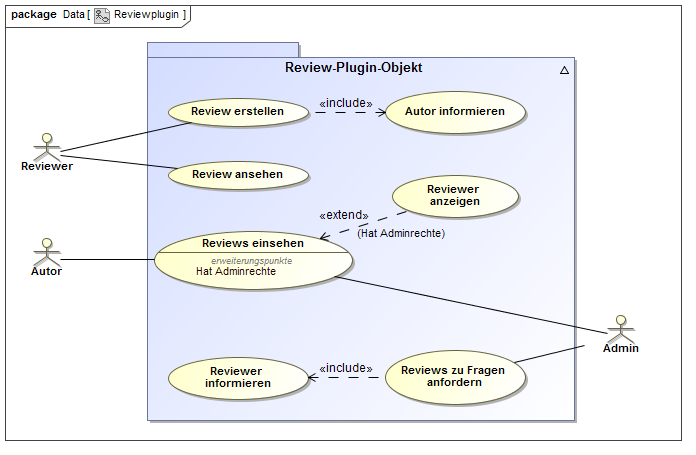
\includegraphics[scale=0.45]{Diagramme/Use_Case_Diagram__Reviewplugin.png}
			\label{Reviewplugin}	
		\end{frame}
		\begin{frame}
			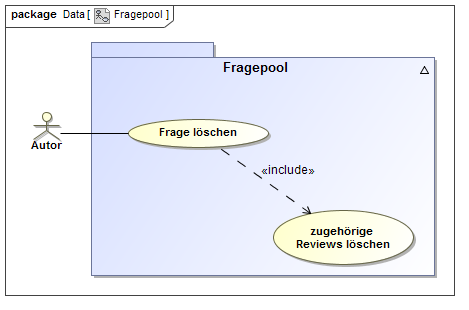
\includegraphics[scale=0.7]{Diagramme/Use_Case_Diagram__Fragepool.png}
				\label{Fragepool}
		\end{frame}
	\section{Probleme}
		\begin{frame}
			\frametitle{Problembehandlung}
    		\begin{itemize}
    			\item Wahl des Repositorys
		    	\item Erstellen der Reviewbaren Fragen
    			\item Wahl der Reviewerzuordnung
    		\end{itemize}
		\end{frame}

	\section{Diagramme und Prototyp}
		
\end{document}